% Packages =====================================================================

\documentclass{article}
\usepackage{nips13submit_e}
\usepackage{times}
\usepackage[utf8]{inputenc}
\usepackage[authoryear]{natbib}
\usepackage{amsmath}
\usepackage{amsthm}
\usepackage{amssymb}
\usepackage{xcolor}
\usepackage{auto-pst-pdf}
\usepackage{pst-plot}
\usepackage{floatrow}
\usepackage[font=small,labelfont=bf]{caption}



% Various settings =============================================================

\newtheorem{theorem}{Theorem}
\newtheorem{lemma}[theorem]{Lemma}
\newtheorem{proposition}[theorem]{Proposition}
\newtheorem{corollary}[theorem]{Corollary}

\usepackage{xr}
\externaldocument{nips-suppl}

\newcommand{\lwh}[1]{\textcolor{blue}{#1}}



% Title ========================================================================

\title{\textbf{Understanding variable importances\\
in forests of randomized trees}}

\author{
Gilles Louppe, Louis Wehenkel, Antonio Sutera and Pierre Geurts\\
Dept. of EE \& CS, University of Liège, Belgium \\
\texttt{\{g.louppe, l.wehenkel, a.sutera, p.geurts\}@ulg.ac.be}\\
% \And
% Louis Wehenkel \\
% University of Liège, Belgium \\
% \texttt{l.wehenkel@ulg.ac.be} \\
% % \And
% % Antonio Sutera \\
% % University of Liège, Belgium \\
% % \texttt{antonio.sutera@student.ulg.ac.be} \\
% \And
% Pierre Geurts \\
% University of Liège, Belgium \\
% \texttt{p.geurts@ulg.ac.be} \\
}


\newcommand{\fix}{\marginpar{FIX}}
\newcommand{\new}{\marginpar{NEW}}

\nipsfinalcopy % Uncomment for camera-ready version

\begin{document}

\maketitle
\allowdisplaybreaks

\begin{abstract}

Despite growing interest and practical use in various scientific areas, variable
importances derived from tree-based ensemble methods are not well understood
from a theoretical point of view. In this work we characterize the Mean Decrease
Impurity (MDI) variable importances as measured by an ensemble of totally
randomized trees in asymptotic sample and ensemble size conditions. We derive a
three-level decomposition of the  information jointly provided by all input
variables about the output in terms of i) the MDI importance of each input
variable, ii) the degree of interaction of a given input variable with the other
input variables, iii) the different interaction terms of a given degree. We then
show that this MDI importance of a variable is equal to zero if and only if the
variable is irrelevant and that the MDI importance of a relevant variable is
invariant with respect to the removal or the addition of irrelevant variables.
We illustrate these properties on a simple example and discuss how they may
change in the case of  non-totally randomized trees such as Random Forests and
Extra-Trees.


\end{abstract}



% Motivation ===================================================================

\section{Motivation}

An important task in many scientific fields is the prediction of  a response
variable based on a set of predictor variables. In many situations though, the
aim is not only to make the most accurate predictions of the response but also
to identify which predictor variables are the most important to make these
predictions, e.g. in order to understand the underlying process. Because of
their applicability to a wide range of problems and their capability to both
build accurate models and, at the same time, to provide variable importance
measures, Random Forests~\citep{breiman2001rf} and variants such as Extra-Trees~\citep{geurts2006et}
have become a major data analysis tool used with
success in various scientific areas.

Despite their extensive use in applied research, only a couple of works have
studied the theoretical properties and statistical mechanisms of these
algorithms. \citet{zhao2000new}, \citet{breiman2004consistency},
\citet{biau2008consistency,biau2012analysis}, \citet{meinshausen2006quantile}
and \citet{lin2006random} investigated simplified to very realistic variants of
these algorithms and proved  the consistency of those variants. Little is known
however regarding the variable importances computed by Random Forests like
algorithms, and -- as far as we know -- the work of~\citet{ishwaran2007variable}
is indeed the only theoretical study of tree-based variable importance measures.

In this work, we aim at filling this gap and present a theoretical  analysis of
the Mean Decrease Impurity importance derived from ensembles of randomized
trees. The rest of the paper is organized as follows: in
section~\ref{sec:background}, we provide  the background about ensembles of
randomized trees and recall how variable importances can be derived from them;
in section~\ref{sec:var-imp}, we then derive a characterization in asymptotic
conditions and show how variable importances derived from totally randomized
trees offer a three-level decomposition of the information jointly contained in
the input variables about the output; section~\ref{sec:rel} shows that this
characterization only depends on the relevant variables and
section~\ref{sec:variants} discusses theses ideas in the context of variants
closer to the Random Forest algorithm; section~\ref{sec:example} then
illustrates all these ideas on an artificial problem; finally,
section~\ref{sec:conclusions} includes our conclusions and proposes directions
of future works.



% Background ===================================================================

\section{Background}
\label{sec:background}

In this section, we first describe decision trees, as well as forests of
randomized trees. Then, we describe the two major variable importances measures
derived from them -- including the Mean Decrease Impurity (MDI) importance that we
will study in the subsequent sections.

\subsection{Single classification and regression trees and random forests}

A binary classification (resp. regression)  tree~\citep{breiman1984cart}
is an input-output model represented by a tree  structure $T$, from a random input
vector $(X_1, ..., X_p)$ taking its values in ${\cal X}_1 \times ... \times
{\cal X}_p = {\cal X}$ to a random output variable $Y\in {\cal Y}$ . Any node  $t$ in
the tree represents a subset of the space ${\cal X}$, with the root node being
${\cal X}$ itself. Internal nodes $t$ are labeled with a binary test (or split)
$s_t = (X_m < c)$ dividing their subset in two subsets\footnote{More generally, splits are defined by a (not necessarily binary)
partition of the range ${\cal X}_{m}$ of possible values of a single variable
$X_{m}$.} corresponding to their two children $t_L$ and
$t_R$, %We respectively note $v(s)=X_m$ and $c(s)=c$ the variable and the discretization threshold used in split $s$.
while the terminal nodes (or leaves) are
labeled with a best guess value of the output variable\footnote{e.g. determined as the majority
class $j(t)$ (resp., the average value $\bar{y}(t)$) within the subset of the leaf $t$.}. The
predicted output $\hat{Y}$ for a new instance is the label
of the leaf reached by the instance when it is propagated through the tree. A  tree
is built from a learning sample of size $N$ drawn from $P(X_1, ..., X_p, Y)$
using a recursive procedure which identifies at each node $t$ the split
$s_t=s^*$ for which the partition of the $N_t$ node samples into $t_L$ and $t_R$
maximizes the decrease
\begin{equation}\label{eq:deltaimpurity}
\Delta i(s, t) = i(t) - p_L i(t_L) - p_R i(t_R)
\end{equation}
of some impurity measure $i(t)$ (e.g., the Gini index, the Shannon entropy, or the variance of $Y$), and where $p_L=N_{t_L} / {N_t}$ and $p_R={N_{t_R}}/{N_t}$. The
construction of the tree stops , e.g., when
nodes become pure in terms of $Y$ or when all variables $X_{i}$ are locally constant.


%\subsection{Forests of randomized trees}

Single trees typically suffer from high variance, which makes them not
competitive in terms of accuracy. A very efficient and simple way to address
this flaw is to use them in the context of randomization-based ensemble methods.
Specifically, the core principle is to introduce random perturbations into the
learning procedure in order to produce several different decision trees from a
single learning set and to use some aggregation technique to combine the predictions of all these trees.  In Bagging~\citep{breiman1996bagging}, trees are built on
random bootstrap copies of the original data, hence producing different decision
trees. In Random Forests~\citep{breiman2001rf}, Bagging is extended and combined
with a randomization of the input variables that are used when considering
candidate variables to split internal nodes $t$. In particular, instead of
looking for the best split $s^*$ among all variables, the Random Forest algorithm selects, at
each node, a random subset of $K$ variables and then determines the best split
over these latter variables only.
%In extremely randomized trees~\citep{geurts2006et},
%randomization goes one step further: discretization threholds $c$ are also
%drawn at random and the best test is chosen among the $K$ randomly drawn cut-
%points. Unlike in random forests though, the trees are not built on bootstrap
%copies of the input data.

\subsection{Variable importances}

% In the context of single decision trees, \cite{breiman1984cart} first defined
% the measure of importance of a variable $X_m$ as $Imp(X_m) = \sum_{t\in T}
% \Delta I(\tilde{s}^m_t, t)$, where $\tilde{s}^m_t$ is the best surrogate split
% for $s_t$ -- that is the best split using variable $X_m$ to predict the actual
% split $s_t$ defined at node $t$. The use of surrogate splits was proposed to
% account for masking effects: it may indeed happen that some variable $X_{m_2}$
% never occurs in any split because it leads to splits that are slightly worse,
% and therefore not selected, than those of some other variable $X_{m_1}$.
% However, if $X_{m_1}$ is removed and another tree is grown, $X_{m_2}$ may now
% occur prominently within the splits and the resulting tree may be nearly as good
% as the original tree. In such a case, a relevant measure should detect the
% importance of $X_{m_2}$. Accordingly, if $X_{m_2}$ is being masked at $t$ by
% $X_{m_1}$ (i.e., if $v(s_t)=X_{m_1}$), but if $\tilde{s}^{m_2}_t$ is similar to
% $s_t$, but not quite as good, then $\Delta I(\tilde{s}^{m_2}_t, t)$ will be
% nearly as large as $\Delta I(s_t, t)$ and therefore the proposed measure will
% indeed account for the importance of $X_{m_2}$.

% Thanks to randomization, masking effects are dampened within forests of
% randomized trees. Even if $X_{m_2}$ is being masked by $X_{m_1}$ there is indeed
% still a chance for $X_{m_2}$ to be chosen as a split if $X_{m_1}$ is not
% selected among the $K$ variables chosen at random. Depending on the value $K$,
% masking effects do not disappear entirely though. The use of bootstrap samples
% also helps reduce masking effects, making $X_{m_1}$ or $X_{m_2}$ just slightly
% better than the other due to the variations in the bootstrap samples.


In the context of ensembles of randomized trees,
\cite{breiman2001rf,breiman2002manual} proposed to evaluate the importance of
a variable $X_m$  for predicting  $Y$ by adding up the weighted impurity decreases $p(t) \Delta
i(s_t, t)$ for all nodes $t$ where $X_m$ is used, averaged over all $N_T$ trees
in the forest:
\begin{equation}\label{eq:mdi}
Imp(X_m) = \frac{1}{N_T} \sum_{T} \sum_{t \in T:v(s_t) = X_m} p(t) \Delta i(s_t, t)
\end{equation}
and where $p(t)$ is the proportion $N_t / N$ of samples
reaching $t$ and $v(s_t)$ is the variable used in split $s_t$. When
using the Gini index as impurity function, this measure is known as the
\textit{Gini importance} or \textit{Mean Decrease Gini}. However, since it can
be defined for any impurity measure $i(t)$, we will refer to Equation~\ref{eq:mdi}
as the \textit{Mean Decrease Impurity} importance (MDI), no matter the impurity
measure $i(t)$. We will characterize and derive results for this measure in the
rest of this text.

In addition to MDI,
\cite{breiman2001rf,breiman2002manual} also proposed to evaluate the importance
of a variable $X_m$ by measuring the \textit{Mean Decrease Accuracy} (MDA) of
the forest when the values of $X_m$ are randomly permuted in the out-of-bag
samples. For that reason, this latter measure is also known as the
\textit{permutation importance}.

Thanks to popular machine learning
softwares~\citep{breiman2002manual,liaw2002classification,pedregosa2011scikit},
both of these variable importance measures have shown their practical utility in
an increasing number of experimental studies. Little is known however regarding
their inner workings. \cite{strobl2007bias} compare both MDI and MDA and show
experimentally that the former is biased towards some predictor variables. As
explained by~\cite{white1994technical} in case of single decision trees, this
bias stems from an unfair advantage given by the usual impurity functions $i(t)$
towards predictors with a large number of values. \cite{strobl2008conditional}
later showed  that MDA is biased as well, and that it overestimates the
importance of correlated variables -- although this effect was not confirmed in
a later experimental study by~\cite{genuer2010variable}.  From a theoretical
point of view, \cite{ishwaran2007variable} provides a detailed theoretical
development of a simplified version of MDA, giving key insights for the
understanding of the actual MDA.




% Characterization of variable importances =====================================

\section{Variable importances derived from totally randomized tree ensembles}
\label{sec:var-imp}

Let us now consider the MDI  importance
as defined by Equation~\ref{eq:mdi}, and let us assume a set $V= \{X_1, ..., X_p\}$  of {\em categorical}
input variables and a {\em categorical} output $Y$. For the sake of
simplicity we will  use the Shannon entropy as impurity measure, and focus on
totally randomized trees; later on we will discuss other impurity measures and tree construction algorithms.

Given a training sample ${\cal L}$ of $N$ joint observations of $X_1, ..., X_p,
Y$ independently drawn from the joint distribution $P(X_1, ..., X_p, Y)$, let us
assume that we infer from it an infinitely large ensemble of \textit{totally
randomized and fully developed trees}. In this setting, a totally randomized and
fully developed tree is defined as a decision tree in which each node $t$ is
partitioned using a variable $X_i$ picked uniformly at random among those not
yet used at the parent nodes of $t$, and where each $t$ is split into $|{\cal
X}_i|$ sub-trees, i.e., one for each possible value of ${\cal X}_i$, and where
the recursive construction process halts only when all $p$ variables have been
used along the current branch.  Hence, in such a tree, leaves are all at the
same depth $p$, and the set of leaves of a fully developed tree is in bijection
with the set $\cal X$ of all possible joint configurations of the $p$ input
variables. For example, if the input variables are all binary, the resulting
tree will have exactly $2^{p}$ leaves.

\begin{theorem}\label{thm:imp}
The MDI importance of $X_m \in V$ for $Y$ as computed
with an   infinite ensemble of fully developed totally randomized trees and an
infinitely large training sample is:
  \begin{equation}\label{eqn:imp-full}
  Imp(X_m)=\sum_{k=0}^{p-1} \frac{1}{C_p^k} \frac{1}{p-k} \sum_{B \in {\cal P}_k(V^{-m})} I(X_m;Y|B),
  \end{equation}
\end{theorem}
\noindent where $V^{-m}$ denotes the subset $V \setminus \{X_m\}$, ${\cal
P}_k(V^{-m})$ is the set of subsets of  $V^{-m}$ of cardinality $k$, and
$I(X_m;Y|B)$ is the conditional mutual information of $X_{m}$ and $Y$ given the
variables in $B$.

\begin{proof}
See Appendix~\ref{app:thm:imp}.
\end{proof}

\begin{theorem}\label{thm:sum-of-imp}
For any ensemble of fully developed trees in asymptotic learning sample size
conditions (e.g., in the same conditions as those of Theorem~\ref{thm:imp}), we
have that
\begin{equation}\label{eqn:sum-of-imp}
\sum_{m=1}^{p}Imp(X_m) = I(X_{1}, \ldots, X_{p} ; Y).
\end{equation}
\end{theorem}

\begin{proof}
See Appendix~\ref{app:thm:sum-of-imp}.
\end{proof}

Together, theorems \ref{thm:imp} and \ref{thm:sum-of-imp} show that  variable
importances derived from totally randomized trees in asymptotic conditions
provide a three-level decomposition of the information $I(X_{1}, \ldots, X_{p}
; Y)$ contained in the set of input variables about the output variable. The
first level is a decomposition among input variables (see Equation~\ref{eqn:sum-of-imp}
of Theorem~\ref{thm:sum-of-imp}),  the second level is a decomposition
along the degrees $k$ of interaction terms of a variable with the other ones
(see the outer sum in Equation~\ref{eqn:imp-full} of Theorem~\ref{thm:imp}), and
the third level is a decomposition along the combinations $B$ of interaction
terms of fixed size $k$ of possible interacting variables (see the inner sum in Equation~\ref{eqn:imp-full}).

We observe that the decomposition includes, for each variable, each and every interaction term
of each and every degree weighted in a fashion resulting only from the
combinatorics of possible interaction terms. In particular, since all
$I(X_m;Y|B)$ terms are at most equal to $H(Y)$, the prior entropy of $Y$,  the
$p$ terms of the outer sum of Equation~\ref{eqn:imp-full} are each upper bounded
by $$\frac{1}{C^k_p}\frac{1}{p-k}\sum_{B \in {\cal P}_k(V^{-m})}
H(Y)=\frac{1}{C^k_p} \frac{1}{p-k} {C^k_{p-1}} H(Y) = \frac{1}{p}H(Y).$$ As such,
the second level decomposition resulting from totally randomized trees makes the
$p$ sub-importance terms $\frac{1}{C^k_p} \frac{1}{p-k} \sum_{B \in {\cal
P}_k(V^{-m})} I(X_m;Y|B)$ to equally contribute (at most) to the total
importance, even though they each include a combinatorially different number of
terms.


% Irrelevant variables =========================================================

\section{Importances of relevant and irrelevant variables}
\label{sec:rel}

Following~\citet{kohavi1997wrappers}, let us define as {\em relevant to $Y$ with
respect to $V$} a variable $X_m$ for which there exists at least one subset $B
\subseteq V$ (possibly empty) such that $I(X_m;Y|B)>0$.\footnote{Among the
relevant variables, we have the {\em marginally} relevant
ones, for which $I(X_{m}; Y) > 0$, the  {\em strongly} relevant ones, for
which $I(X_{m}; Y | V^{-m}) > 0$,  and the {\em weakly} relevant variables, which are
relevant but not strongly relevant. } Thus we define as {\em irrelevant to $Y$ with respect to $V$} a variable
$X_i$ for which, for all $B \subseteq V$, $I(X_i; Y|B)=0$. Remark that if
$X_i$ is irrelevant to $Y$ with respect to $V$, then by definition it is also
irrelevant to $Y$ with respect to any subset of $V$. %However, if $X_m$ is relevant to $Y$ with
%respect to $V$, then it is not necessarily relevant to $Y$ with respect to all  subsets
%of $V$.

\begin{theorem}\label{thm:irrelevant}
  $X_i \in V$ is irrelevant to $Y$ with respect to $V$ if and only if  its
  infinite sample size importance as computed with an infinite ensemble of fully
  developed totally randomized trees built on $V$ for $Y$ is 0.
\end{theorem}

\begin{proof}
See Appendix~\ref{app:thm:irrelevant}.
\end{proof}

\begin{lemma}\label{lemma:adding-irrelevant}
  Let $X_i \notin V$ be an irrelevant variable for $Y$ with respect to $V$. The infinite
  sample size importance of $X_m \in V$ as computed with an infinite
  ensemble of fully developed totally randomized trees built on $V$ for $Y$ is the
  same as the importance derived when using $V\cup \{X_i\}$ to build the ensemble of trees for $Y$.
\end{lemma}

\begin{proof}
See Appendix~\ref{app:lemma:adding-irrelevant}.
\end{proof}

\begin{theorem}\label{thm:relevant}
  Let $V_R \subseteq V$ be the subset of all variables in $V$ that are relevant to $Y$ with
  respect to $V$. The infinite sample size importance of any variable $X_m \in
  V_R$ as computed with an infinite ensemble of fully developed totally randomized
  trees built on $V_R$ for $Y$ is the same as its importance computed in the same conditions by using all variables in $V$. That is:
    \begin{equation}
      \begin{aligned}
      Imp(X_m)&=\sum_{k=0}^{p-1} \frac{1}{C_p^k} \frac{1}{p-k} \sum_{B \in {\cal P}_k(V^{-m})} I(X_m;Y|B)\\
              &=\sum_{l=0}^{r-1} \frac{1}{C_r^l} \frac{1}{r-l} \sum_{B \in {\cal P}_l(V_R^{-m})} I(X_m;Y|B)\\
      \end{aligned}
    \end{equation}
  where $r$ is the number of relevant variables in $V_R$.
\end{theorem}


\begin{proof}
See Appendix~\ref{app:thm:relevant}.
\end{proof}

Theorems~\ref{thm:irrelevant} and \ref{thm:relevant} show that the
importances computed with an ensemble of totally randomized trees depends only
on the relevant variables. Irrelevant variables have a zero importance and do
not affect the importance of relevant variables. Practically, we believe that
such properties are desirable conditions for a sound criterion assessing the
importance of a variable. Indeed, noise should not be credited of any importance
and should not make any other variable more (or less) important.

%Intuitively, the independence with respect to irrelevant variables can be partly
%attributed to the fact that splitting at $t$ on some irrelevant variable $X_i$
%should only dillute the local importance $p(t) \Delta i(t)$ of a relevant
%variable $X_m$ into the children $t_L$ and $t_R$, but not affect the total sum.
%For instance, if $X_m$ was to be used at $t$, then the local importance would be
%proportional to $p(t)$. By contrast, if $X_i$ was to be used at $t$ and $X_m$ at
%$t_L$ and $t_R$, then the sum of the local importances for $X_m$ would be
%proportional to $p(t_L) + p(t_R)=p(t)$, which does not change anything.
%Similarly, one can recursively invoke the same argument if $X_m$ was to be used
%deeper in $t_L$ or $t_R$.

% A second reason comes from the
% fact that local importances are collected only in nodes $t$ where $X_m$ is used.
% By contrast, if local importances were summed over all nodes (e.g., using
% surrogate splits), then it would necessarily depend on the total number of nodes
% in a tree, which itself directly depends on $p$ -- that is, not on $r$.

% Finally, it is also worth noting that this result is consistent with the work
% of~\citet{biau2012analysis}, who proved that rate of convergence of forests
% of randomized also only depends on the relevant variables.



% Extensions ===================================================================

\section{Random Forest variants}
\label{sec:variants}

In this section, we consider and discuss variable importances as computed with
other types of ensembles of randomized trees. We first show how our results extend to any other impurity measure, and then analyze importances computed by depth-pruned ensemble of randomized trees and those
computed by randomized trees built on random subspaces of fixed size. Finally, we
discuss the case of non-totally randomized trees.

\subsection{Generalization to other impurity measures}

Although our characterization in sections~\ref{sec:var-imp} and
\ref{sec:rel} uses Shannon entropy as the impurity measure, we show in
Appendix~\ref{app:generalization} that theorems~\ref{thm:imp},
\ref{thm:irrelevant} and \ref{thm:relevant} hold for other impurity
measures, simply substituting conditional mutual information for
conditional impurity reduction in the different formulas and in
the definition of irrelevant variables.  In particular, our results
thus hold for the Gini index in classification and can be extended to
regression problems using variance as the impurity measure.

%\textcolor{red}{Expliquer en quelques mots que cela tient à la définition d'irrelevance qu'on considère.}




% Pruning and RS ---------------------------------------------------------------

\subsection{Pruning and random subspaces}

In sections~\ref{sec:var-imp} and \ref{sec:rel}, we considered totally randomized trees that were
fully developed, i.e. until all $p$ variables were used within each branch. When
totally randomized trees are developed only up to some smaller depth $q \leq p$,
we show in Proposition~\ref{proposition:pruning} that the variable importances
as computed be these trees is limited to the $q$ first terms of
Equation~\ref{eqn:imp-full}. We then show in Proposition~\ref{proposition:imp-subspaces}
that these latter importances are actually the same as when each tree
of the ensemble is fully developed over a random subspace~\citep{ho1998random}
of $q$ variables drawn prior to its construction.

\begin{proposition}\label{proposition:pruning}
  The importance of $X_m \in V$ for $Y$ as computed with an
  infinite ensemble of pruned totally randomized trees built up to depth $q \leq p$ and an
infinitely large training sample is:
  \begin{equation}\label{eqn:imp-pruning}
  Imp(X_m)=\sum_{k=0}^{q-1} \frac{1}{C_p^k} \frac{1}{p-k} \sum_{B \in {\cal P}_k(V^{-m})} I(X_m;Y|B)
  \end{equation}
\end{proposition}

\begin{proof}
See Appendix~\ref{app:proposition:pruning}.
\end{proof}

\begin{proposition}\label{proposition:imp-subspaces}
  The importance of $X_m \in V$ for $Y$ as computed with an infinite ensemble   of
pruned totally randomized trees built up to depth $q \leq p$ and an infinitely
large training sample is identical to the importance as computed  for $Y$ with an
infinite ensemble of fully developed totally randomized trees built on random
subspaces of $q$ variables drawn from $V$.
\end{proposition}

\begin{proof}
See Appendix~\ref{app:proposition:imp-subspaces}.
\end{proof}

As long as $q  \geq r $ (where $r$ denotes the number of relevant variables in $V$), it can easily be shown that all relevant variables
will still obtain a strictly positive importance, which will however differ in
general from the importances computed by fully grown totally randomized trees
built over all variables.  Also, each irrelevant variable of course keeps an
importance equal to zero, which means that, in asymptotic conditions, these
pruning and random subspace methods would still allow us identify the relevant  variables, as long as we
have a good upper bound $q$ on $r$.



% Non-totally randomized trees -------------------------------------------------

\subsection{Non-totally randomized trees}
\label{sec:ntrt}

In our analysis in the previous sections, trees are built totally at random and hence do not directly relate
to those built in Random Forests~\citep{breiman2001rf} or in Extra-Trees~\citep{geurts2006et}. To better understand the importances as
computed by those algorithms,  let us consider a close variant of totally
randomized trees: at each node $t$, let us instead draw uniformly at random $1
\leq K \leq p$ variables  and let us choose the one that maximizes $\Delta i(t)$.
%As previously, $t$ is split into as many subtrees as the cardinality of the
%chosen variable. Asymptotically, for binary variables, this variant exactly
%matches random forests and extremely randomized trees.
%For variables with a larger cardinality, the correspondance no longer exactly holds but the trees still closely relate.
Notice that, for $K=1$, this
procedure amounts to building ensembles of  totally randomized trees as defined before, while,
for $K=p$, it amounts to building classical single trees in a deterministic way.

First, the importance of  $X_m \in V$ as computed with an infinite ensemble of
such randomized trees is not the same as Equation~\ref{eqn:imp-full}. For $K>1$,
masking effects indeed appear: at $t$, some variables are never selected
because there always is some other variable for which $\Delta i(t)$ is larger.
Such effects tend to pull the best variables  at the top of the trees and to
push the others at the leaves.  As a result, the importance of a variable no
longer decomposes into a sum including all $I(X_m;Y|B)$ terms. The
importance of the best variables decomposes into a sum of their mutual
information alone or conditioned only with the best others -- but not
conditioned with all variables since they no longer ever appear at the bottom of
trees. By contrast, the importance of the least promising variables now
decomposes into a sum of their mutual information conditioned only with all
variables -- but not alone or conditioned with a couple of others since they no
longer ever appear at the top of trees. In other words, because of the guided
structure of the trees, the importance of $X_m$ now takes into account only some
of the conditioning sets $B$, which may over- or underestimate its overall
relevance.

To make things clearer, let us consider a simple example. Let $X_1$ perfectly explains $Y$
 and let $X_2$ be a slightly noisy copy of $X_1$ (i.e., $I(X_1;Y)
\approx I(X_2;Y)$, $I(X_1;Y|X_2)=\epsilon$ and $I(X_2;Y|X_1)=0$). Using totally
randomized trees, the importances of $X_1$ and $X_2$ are nearly equal -- the
importance of $X_1$ being slightly higher than the importance of $X_2$:
\begin{eqnarray*}
Imp(X_1) &=& \frac{1}{2} I(X_1;Y) + \frac{1}{2} I(X_1;Y|X_2) = \frac{1}{2} I(X_1;Y) + \frac{\epsilon}{2}\\
Imp(X_2) &=& \frac{1}{2} I(X_2;Y) + \frac{1}{2} I(X_2;Y|X_1) = \frac{1}{2} I(X_2;Y) + 0
\end{eqnarray*}
In non-totally randomized trees, for $K=2$, $X_1$ is always selected at the root
node and $X_2$ is always used in its children. Also, since $X_1$ perfectly
explains $Y$, all its children are pure and the reduction of entropy when
splitting on $X_2$ is null. As a result, $Imp_{K=2}(X_1) = I(X_1;Y)$ and
$Imp_{K=2}(X_2) = I(X_2;Y|X_1) = 0$. Masking effects are here
clearly visible: the true importance of $X_2$ is masked by $X_1$ as if $X_2$
were irrelevant, while it is only a bit less informative than $X_1$.

As a direct consequence of the example above, for $K>1$, it is no longer true
that a variable is irrelevant if and only if its importance is zero. In the same
way, it can also be shown that the importances become dependent on the number of
irrelevant variables. Let us indeed consider the following counter-example: let
us add in the previous example an irrelevant variable $X_i$ with respect to
$\{X_1, X_2\}$ and let us keep $K=2$. The probability of selecting $X_2$ at the
root node now becomes positive, which means that $Imp_{K=2}(X_2)$ now includes
$I(X_2;Y)>0$ and is therefore strictly larger than the importance computed
before. For $K$ fixed, adding irrelevant variables dampens masking effects,
which thereby makes importances indirectly dependent on the number of irrelevant
variables.

In conclusion, the importances as computed with totally randomized trees
exhibit properties that do not possess, by extension, neither random forests nor
extra-trees. With totally randomized trees, the importance of
$X_m$ only depends on the relevant variables and is 0 if and only if $X_m$ is
irrelevant. As we have shown, it may no longer be the case for $K>1$.
Asymptotically, the use of totally randomized trees for assessing the importance of
a variable may therefore be more appropriate. In a finite setting (i.e., a
limited number of samples and a limited number of trees), guiding the choice of
the splitting variables remains however a sound strategy. In such a case,
$I(X_m;Y|B)$ cannot be measured neither for all $X_m$ nor for all $B$. It is
therefore  pragmatic to promote those that look the most promising -- even if
the resulting importances may be biased.


% Impurity measures ------------------------------------------------------------


% Experiments ==================================================================

\section{Illustration on a digit recognition problem}
\label{sec:example}

In this section, we consider the digit recognition
problem of \citep{breiman1984cart} for illustrating variable importances as
computed with totally randomized trees. We verify that they match with our
theoretical developments and that they decompose as foretold. We also compare
these importances with those computed by an ensemble of non-totally randomized
trees, as discussed in section~\ref{sec:ntrt}, for increasing values of $K$.

Let us consider a seven-segment indicator displaying numerals using horizontal and
vertical lights in on-off combinations, as illustrated in
Figure~\ref{fig:digits}. Let $Y$ be a random variable taking its value in $\{0, 1,
..., 9\}$ with equal probability and  let $X_1, ..., X_7$ be binary variables
whose values are each determined univocally given the corresponding value of $Y$
in Table~\ref{table:digits}.

\begin{figure*}\RawFloats
\begin{minipage}[b]{\textwidth}
  \begin{minipage}[b]{0.4\textwidth}
    \centering
    \begin{pspicture}(0,0)(2.0,4.0)
        \usefont{T1}{ptm}{m}{n}
        \psline[linewidth=0.02cm](0.0,0.0)(0.0,0.7)
        \psline[linewidth=0.02cm](0.0,0.0)(0.7,0.0)
        \psline[linewidth=0.02cm](2.0,0.0)(2.0,0.7)
        \psline[linewidth=0.02cm](2.0,0.0)(1.3,0.0)
        \psline[linewidth=0.02cm](0.0,2.0)(0.0,1.3)
        \psline[linewidth=0.02cm](0.0,2.0)(0.7,2.0)
        \psline[linewidth=0.02cm](2.0,2.0)(2.0,1.3)
        \psline[linewidth=0.02cm](2.0,2.0)(1.3,2.0)
        \psline[linewidth=0.02cm](0.0,2.0)(0.0,2.7)
        \psline[linewidth=0.02cm](2.0,2.0)(2.0,2.7)
        \psline[linewidth=0.02cm](0.0,4.0)(0.0,3.3)
        \psline[linewidth=0.02cm](0.0,4.0)(0.7,4.0)
        \psline[linewidth=0.02cm](2.0,4.0)(2.0,3.3)
        \psline[linewidth=0.02cm](2.0,4.0)(1.3,4.0)
        \rput(1.0,4.0){$X_1$}
        \rput(0.0,3.0){$X_2$}
        \rput(2.0,3.0){$X_3$}
        \rput(1.0,2.0){$X_4$}
        \rput(0.0,1.0){$X_5$}
        \rput(2.0,1.0){$X_6$}
        \rput(1.0,0.0){$X_7$}
    \end{pspicture}
    \captionof{figure}{7-segment display}
    \label{fig:digits}
  \end{minipage}
  \hfill
  \begin{minipage}[b]{0.58\textwidth}
    \centering
    \begin{tabular}{ c | c c c c c c c }
    \hline
    $y$ & $x_1$ & $x_2$ & $x_3$ & $x_4$ & $x_5$ & $x_6$ & $x_7$ \\
    \hline
    0 & 1 & 1 & 1 & 0 & 1 & 1 & 1 \\
    1 & 0 & 0 & 1 & 0 & 0 & 1 & 0 \\
    2 & 1 & 0 & 1 & 1 & 1 & 0 & 1 \\
    3 & 1 & 0 & 1 & 1 & 0 & 1 & 1 \\
    4 & 0 & 1 & 1 & 1 & 0 & 1 & 0 \\
    5 & 1 & 1 & 0 & 1 & 0 & 1 & 1 \\
    6 & 1 & 1 & 0 & 1 & 1 & 1 & 1 \\
    7 & 1 & 0 & 1 & 0 & 0 & 1 & 0 \\
    8 & 1 & 1 & 1 & 1 & 1 & 1 & 1 \\
    9 & 1 & 1 & 1 & 1 & 0 & 1 & 1 \\
    \hline
    \end{tabular}
    \captionof{table}{Values of $Y, X_1, ..., X_7$}
    \label{table:digits}
  \end{minipage}
\end{minipage}
\end{figure*}

Since Table~\ref{table:digits} perfectly defines the data distribution, and
given the small dimensionality of the problem, it is practicable to directly
apply Equation~\ref{eqn:imp-full} to compute variable importances. To verify our
theoretical developments, we then compare in Table~\ref{table:imp} variable
importances as computed by Equation~\ref{eqn:imp-full} and those yielded by an
ensemble of $10000$ totally randomized trees ($K=1$). Note that given the  known
structure of the problem, building trees on a sample of finite size  that
perfectly follows the data distribution amounts to building them on a sample of
infinite size. At best, trees can thus be built on a 10-sample dataset,
containing exactly one sample for each of the equiprobable outcomes of $Y$. As
the table illustrates, the importances yielded by totally randomized trees match
those computed by Equation~\ref{eqn:imp-full}, which confirms
Theorem~\ref{thm:imp}. Small differences stem from the fact that a finite number
of  trees were built in our simulations, but those discrepancies should
disappear as the size of the ensemble grows towards infinity. It also shows that
importances indeed add up to $I(X_1, ... X_7;Y)$, which confirms
Theorem~\ref{thm:sum-of-imp}.
Regarding the actual importances, they indicate that $X_5$ is stronger than all
others, followed -- in that order -- by $X_2$, $X_4$ and $X_3$ which also show
large importances. $X_1$, $X_7$ and $X_6$ appear to be the less informative. The
table also reports importances for increasing values of $K$. As discussed before,
we see that a large value of $K$ yields importances that can be either
overestimated (e.g., at $K=7$, the importances of $X_2$ and $X_5$ are larger
than at $K=1$) or underestimated due to masking effects (e.g., at $K=7$, the
importances of $X_1$, $X_3$, $X_4$ and $X_6$ are smaller than at $K=1$, as if
they were less important). It can also be observed that masking effects may even
induce changes in the variable rankings (e.g., compare the rankings at $K=1$ and
at $K=7$), which thus confirms that importances are differently affected.

\begin{table}
    \begin{tabular}{ c | c c c c c c c c }
    \hline
        & Eqn.~\ref{eqn:imp-full} & $K=1$ & $K=2$ & $K=3$ & $K=4$ & $K=5$ & $K=6$ & $K=7$ \\
    \hline
    $X_1$ & 0.412 & 0.414 & 0.362 & 0.327 & 0.309 & 0.304 & 0.305 & 0.306\\
    $X_2$ & 0.581 & 0.583 & 0.663 & 0.715 & 0.757 & 0.787 & 0.801 & 0.799\\
    $X_3$ & 0.531 & 0.532 & 0.512 & 0.496 & 0.489 & 0.483 & 0.475 & 0.475\\
    $X_4$ & 0.542 & 0.543 & 0.525 & 0.484 & 0.445 & 0.414 & 0.409 & 0.412\\
    $X_5$ & 0.656 & 0.658 & 0.731 & 0.778 & 0.810 & 0.827 & 0.831 & 0.835\\
    $X_6$ & 0.225 & 0.221 & 0.140 & 0.126 & 0.122 & 0.122 & 0.121 & 0.120\\
    $X_7$ & 0.372 & 0.368 & 0.385 & 0.392 & 0.387 & 0.382 & 0.375 & 0.372\\
    \hline
    $\sum$& 3.321 & 3.321 & 3.321 & 3.321 & 3.321 & 3.321 & 3.321 & 3.321\\
    \hline
    \end{tabular}
    \captionof{table}{Variable importances as computed with an ensemble of randomized trees, for increasing values of $K$. Importances at $K=1$ follow their theoretical values, as predicted by Equation~\ref{eqn:imp-full} in Theorem~\ref{thm:imp}. However, as $K$ increases,  importances diverge due to masking effects. In accordance with Theorem~\ref{thm:sum-of-imp}, their sum is also always equal to $I(X_{1}, \ldots, X_{7}; Y) = H(Y) = \log_{2}(10)= 3.321$ since inputs allow to perfectly predict the output.}
    \label{table:imp}
\end{table}

\begin{figure}
    \centering
    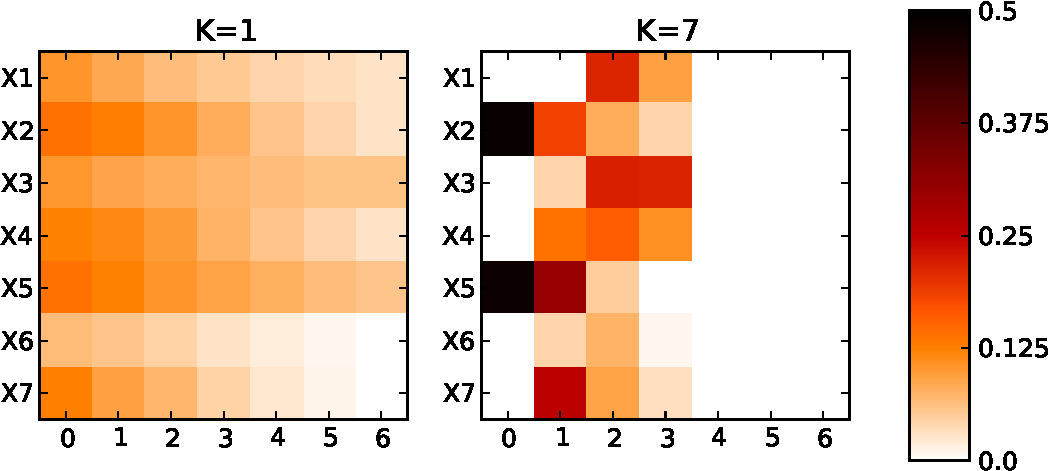
\includegraphics[scale=0.5]{imp-led.pdf}
    \caption{Decomposition of variable importances along the degrees $k$ of interactions of one variable with the other ones. At $K=1$, all $I(X_m;Y|B)$ are accounted for in the total importance, while at $K=7$ only some of them are taken into account due to masking effects.}
    \label{fig:decomposition}
\end{figure}


To better understand why a variable is important, it is also insightful to look
at its decomposition into its $p$ sub-importances terms, as shown in
Figure~\ref{fig:decomposition}. Each row in the plots of the figure corresponds
to one the $p=7$ variables and each column to a size $k$ of conditioning sets.
As such, the value at row $m$ and column $k$ corresponds the importance of $X_m$
when conditioned with $k$ other variables (e.g., to the term $\frac{1}{C^k_p}
\frac{1}{p-k} \sum_{B \in {\cal P}_k(V^{-m})} I(X_m;Y|B)$ in Equation~\ref{eqn:imp-full}
in the case of totally randomized trees). In the left plot, for
$K=1$, the figure first illustrates how importances yielded by totally
randomized trees decomposes along the degrees $k$ of interactions terms. We can
observe that they each equally contribute (at most) the total importance of a
variable. The plot also illustrates why $X_5$ is important: it is informative
either alone or conditioned with any combination of the other variables (all of
its terms are significantly larger than $0$). By contrast, it also clearly shows
why $X_6$ is not important: neither alone nor combined with others $X_6$ seems
to be very informative (all of its terms are close to $0$). More interestingly,
this figure also highlights redundancies: $X_7$ is informative alone or
conditioned with a couple of others (the first terms are significantly larger
than $0$), but becomes uninformative  when conditioned with
many others (the last terms are closer to $0$). The right plot, for $K=7$,
illustrates the decomposition of importances when variables are chosen in a
deterministic way. The first thing to notice is masking effects. Some of the
$I(X_m;Y|B)$ terms are indeed clearly never encountered and their contribution
is therefore reduced to $0$ in the total importance. For instance, for $k=0$,
the sub-importances of $X_2$ and $X_5$ are positive, while all others are null,
which means that only those two variables are ever selected at the root node,
hence masking the others. As a consequence, this also means that the importances
of the remaining variables is biased and that it actually only accounts of their
relevance when conditioned to $X_2$ or $X_5$, but not of their relevance in
other contexts. At $k=0$, masking effects also amplify the contribution of $I(X_2;Y)$
(resp. $I(X_5;Y)$) since $X_2$ (resp. $X_5$) appears more frequently at the root
node than in totally randomized trees. In addition, because nodes become pure
before reaching depth $p$, conditioning sets of size $k\geq4$ are never actually
encountered, which means that we can no longer know whether variables are still
informative when conditioned to many others. All in all, this figure thus indeed
confirms that importances as computed with non-totally randomized trees take
into account only some of the conditioning sets $B$, hence biasing the measured
importances.


% Conclusions ========================================================

\section{Conclusions}
\label{sec:conclusions}

In this work, we made a first step towards understanding variable importances as
computed with a forest of randomized trees. In particular, we derived a
theoretical characterization of the Mean Decrease Impurity importances as
computed by totally randomized trees in asymptotic  conditions.  We showed that
they offer a three-level decomposition of the information jointly provided by
all input variables about the output (Section~\ref{sec:var-imp}). We then demonstrated
(Section~\ref{sec:rel}) that MDI importances as computed by totally randomized
trees exhibit desirable properties for  assessing the relevance of a variable:
it is equal to zero if and only if the variable is irrelevant and it depends
only on the relevant variables. We discussed the case of Random Forests and
Extra-Trees (Section~\ref{sec:variants}) and finally illustrated our
developments on an artificial but insightful example (Section~\ref{sec:example}).

There remain several limitations to our framework that we would like address in
the future. First, our results should be adapted to binary splits as used within
an actual Random Forest-like algorithm. In this setting, any node $t$ is split
in only two subsets, which means that any variable may then appear one or
several times within a branch, and thus should make variable importances now
dependent on the cardinalities of the input variables. In the same direction,
our framework should also be extended to the case of continuous variables.
Finally, results presented in this work are valid in an asymptotic setting only.
An important direction of future work includes the characterization of the
distribution of variable importances in a finite setting.


\medskip \noindent {\small \textbf{Acknowledgements.} GL and PG are respectively
research fellow and research associate of the FNRS, Belgium. This work is
supported by PASCAL2 and the IUAP DYSCO, initiated by the Belgian State, Science
Policy Office.}


% References ===================================================================

\clearpage
\bibliographystyle{apalike}
\bibliography{bib}
\vfill


\end{document}
